\documentclass[
  bibliography=totoc,     % Literatur im Inhaltsverzeichnis
  captions=tableheading,  % Tabellenüberschriften
  titlepage=firstiscover, % Titelseite ist Deckblatt
]{scrartcl}

% Paket float verbessern
\usepackage{scrhack}

% Warnung, falls nochmal kompiliert werden muss
\usepackage[aux]{rerunfilecheck}

% unverzichtbare Mathe-Befehle
\usepackage{amsmath}
% viele Mathe-Symbole
\usepackage{amssymb}
% Erweiterungen für amsmath
\usepackage{mathtools}

% Fonteinstellungen
\usepackage{fontspec}
% Latin Modern Fonts werden automatisch geladen
% Alternativ:
%\setromanfont{Libertinus Serif}
%\setsansfont{Libertinus Sans}
%\setmonofont{Libertinus Mono}
\recalctypearea % Wenn man andere Schriftarten gesetzt hat,
% sollte man das Seiten-Layout neu berechnen lassen

% deutsche Spracheinstellungen
\usepackage{polyglossia}
\setmainlanguage{german}


\usepackage[
  math-style=ISO,    % ┐
  bold-style=ISO,    % │
  sans-style=italic, % │ ISO-Standard folgen
  nabla=upright,     % │
  partial=upright,   % ┘
  warnings-off={           % ┐
    mathtools-colon,       % │ unnötige Warnungen ausschalten
    mathtools-overbracket, % │
},                       % ┘
]{unicode-math}

% traditionelle Fonts für Mathematik
\setmathfont{Latin Modern Math}
% Alternativ:
%\setmathfont{Libertinus Math}

\setmathfont{XITS Math}[range={scr, bfscr}]
\setmathfont{XITS Math}[range={cal, bfcal}, StylisticSet=1]

% Zahlen und Einheiten
\usepackage[
locale=DE,                   % deutsche Einstellungen
separate-uncertainty=true,   % immer Fehler mit \pm
per-mode=symbol-or-fraction, % / in inline math, fraction in display math
]{siunitx}

% chemische Formeln
\usepackage[
version=4,
math-greek=default, % ┐ mit unicode-math zusammenarbeiten
text-greek=default, % ┘
]{mhchem}

% richtige Anführungszeichen
\usepackage[autostyle]{csquotes}

% schöne Brüche im Text
\usepackage{xfrac}

% Standardplatzierung für Floats einstellen
\usepackage{float}
\floatplacement{figure}{htbp}
\floatplacement{table}{htbp}

% Floats innerhalb einer Section halten
\usepackage[
section, % Floats innerhalb der Section halten
below,   % unterhalb der Section aber auf der selben Seite ist ok
]{placeins}

% Seite drehen für breite Tabellen: landscape Umgebung
\usepackage{pdflscape}

% Captions schöner machen.
\usepackage[
  labelfont=bf,        % Tabelle x: Abbildung y: ist jetzt fett
  font=small,          % Schrift etwas kleiner als Dokument
  width=0.9\textwidth, % maximale Breite einer Caption schmaler
]{caption}
% subfigure, subtable, subref
\usepackage{subcaption}

% Grafiken können eingebunden werden
\usepackage{graphicx}
% größere Variation von Dateinamen möglich
\usepackage{grffile}

% schöne Tabellen
\usepackage{booktabs}

% Verbesserungen am Schriftbild
\usepackage{microtype}

% Literaturverzeichnis
\usepackage[style=alphabetic,]{biblatex}
% Quellendatenbank
\addbibresource{lit.bib}
\addbibresource{programme.bib}

% Hyperlinks im Dokument
\usepackage[
  unicode,        % Unicode in PDF-Attributen erlauben
  pdfusetitle,    % Titel, Autoren und Datum als PDF-Attribute
  pdfcreator={},  % ┐ PDF-Attribute säubern
  pdfproducer={}, % ┘
]{hyperref}
% erweiterte Bookmarks im PDF
\usepackage{bookmark}

% Trennung von Wörtern mit Strichen
\usepackage[shortcuts]{extdash}

\title{V504: Thermische Elektronenemission}
\author{
  Simon Schulte
  \texorpdfstring{
    \\
    \href{mailto:simon.schulte@udo.edu}{simon.schulte@udo.edu}
  }{}
  \texorpdfstring{\and}{, }
  Tim Sedlaczek
  \texorpdfstring{
    \\
    \href{mailto:tim.sedlaczek@udo.edu}{tim.sedlaczek@udo.edu}
  }{}
}
\publishers{TU Dortmund – Fakultät Physik}

\date{Durchführung: 23.05.2017\\
      Abgabe: 30.05.2017}


\begin{document}

\maketitle
\thispagestyle{empty}
\tableofcontents
\newpage
\setcounter{page}{1}
\section{Zielsetzung}
\label{sec:zielsetzung}
Ziel des Versuchs ist es, durch Erwärmung einer Metallfläche, freie Elektronen aus dieser zu emittieren.
\section{Theorie}
\label{sec:theorie}
Die durch erhitzung hervorgerufene Elektronenemmision aus einer Metallfläche wird auch als glühelektrischer Effekt bezeichnet. Die Grundlage, um diesen Effekt zu beobachten ist die Austrittsarbeit der Metalloberfläche zu überwinden. Die innere Energie der Elektronen muss somit etwa gleich groß wie die Austrittsarbeit sein, damit diese die Metalloberfläche verlassen können. Dieser Effekt ist temperaturabhängig. Daher werden in diesem Versuch fünf Kennlinien mit fünf verschiedenen Heizströmen und Heizzspannungen aufgenommen.
\begin{figure}[htb]
  \centering
  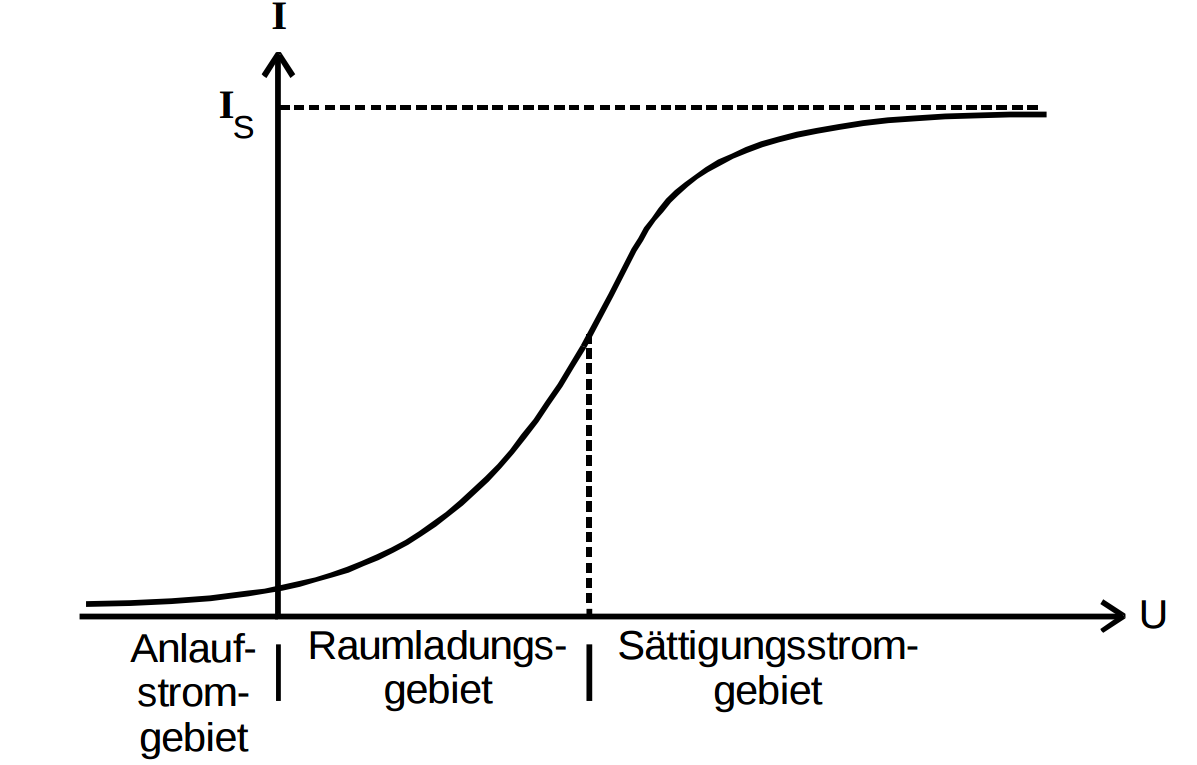
\includegraphics[width=0.9\textwidth]{V5044.png}
  \caption{Der Graph einer Kennlinie. \cite{anleitung}}
  \label{fig:V5044}
\end{figure}
\noindent
Abbildung \ref{fig:V5044} zeigt eine übliche Kennlinie. Dabei wird prinzipiell  die Spannung zwischen Anode und Kathode gegen den fließenden Strom abgebildet. Logischerweise muss das Experiment in einem Vakuum durchgeführt werden, da sonst Teilchen miteinander wechselwirken könnten und somit die Messungen verfälschen würden. Abbildung \ref{fig:V5045} zeigt den Aufbau einer in diesem Versuch verwendeten Diode.
\begin{figure}[H]
  \centering
  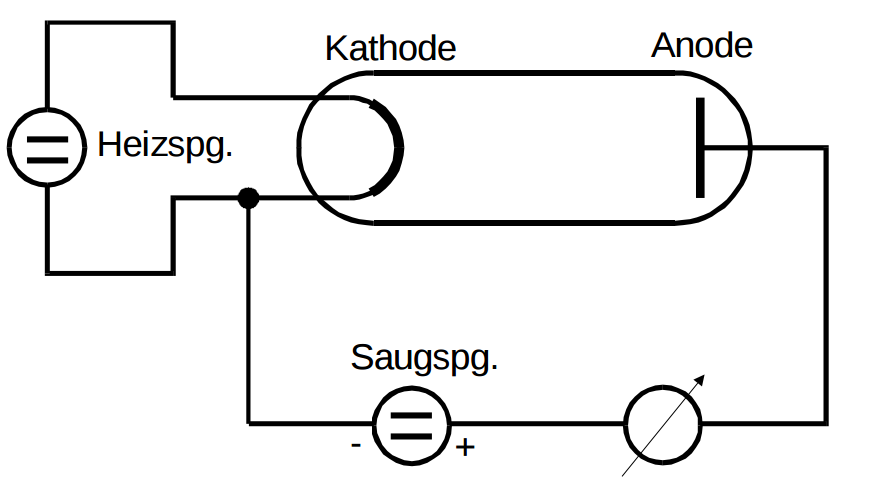
\includegraphics[width=0.9\textwidth]{V5045.png}
  \caption{Der Versuchsaufbau einer Hochvakuumdiode. \cite{anleitung}}
  \label{fig:V5045}
\end{figure}
\noindent
Zu sehen ist, dass der Graph in Abbildung \ref{fig:V5044} drei Teilgebiete aufgeteilt ist. Zum ersten das Anlaufstromgebiet, indem selbst für kleine Gegenspannungen noch ein Anodenstom vorgewiesen werden kann. Dieser Effekt ist darauf zurückzuführen, dass die Elektronen eine Eigengeschwindigkeit beim Verlassen der Kathode besitzen. Dabei ergibt sich für die Stromdichte der Gegenspannung $V$ der Zusammenhang
\begin{equation}
  j(V)\,=\,const\,\exp\Big(-\frac{e_0V}{kT}\Big).
  \label{eqn:stromdichte}
\end{equation}
Nach dem Anlaufstromgebiet folgt das Raumladungsgebiet. Nach der Gleichung
\begin{equation}
  j_\mathup{S} (T)\,=\,4\pi \frac{e_0 m_0 k²}{h³} T² exp\Big(-\frac{e_0 \phi}{kT}\Big)
  \label{eqn:richardson}
\end{equation}
ist die Zahl der pro Zeiteinheit emittierten Elektronen nicht von der Anodenspannung abhängig, sondern lediglich von der Temperatur. Dadurch ist das Raumladungsgebiet nicht für beliebig hohe Anodenspannungen gültig. Die Stromdichte $j$ ist an jeder Stelle konstant und gegeben durch
\begin{equation}
  j\,=\,-\rho v.
  \label{eqn:j}
\end{equation}
Aufgrund der ortsabhängigen Geschwindigkeitsverteilung ergibt sich damit auch eine
ortsabhängige Raumladungsdichte.
Daraus folgt, dass die Raumladungsdichte $\rho$ den Verlauf der Feldstärke zwischen Anode und Kathode beeinflusst. Daher gilt das Langmuir-Schottkysche Raumladungsgesetz:
\begin{equation}
  j\,=\,\frac{4}{9} \epsilon_0 \sqrt{\frac{2e_0}{m_0}}\,\frac{V^{\frac{3}{2}}}{a^2}.
  \label{eqn:raumladung}
\end{equation}
\noindent
Durch eine wachsende Gegenspannung wird der Anodenstrom einem Sättigungswert zustreben. Das darauffolgende Gebiet nennt sich dann Sättigungsstromgebiet. In diesem Bereich erreichen alle Elektronen die Anode.
\section{Durchführung}
\label{sec:durchführung}
\subsection{Versuchsaufbau}
\label{sec:aufbau}
Abbildung \ref{fig:V5041} zeigt den Versuchsaufbau zur Aufnahme der Kennlinien.
Die Kathode der Diode wird dafür durch den Heizstrom erwärmt. Dadurch emittiert diese dann Elektronen, die mit Hilfe der Anodenspannung $U_A$ dann zur Anode gelangen.
\begin{figure}[H]
  \centering
  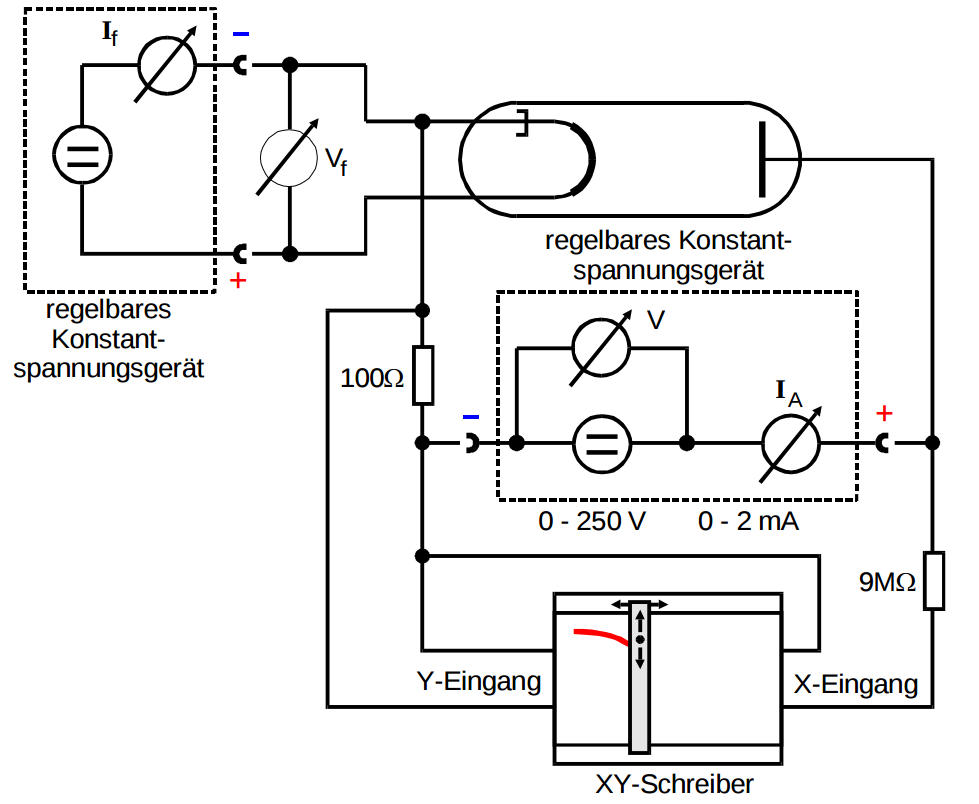
\includegraphics[width=0.9\textwidth]{V5041.png}
  \caption{Der Versuchsaufbau zur Aufnahme der Kennlinien. \cite{anleitung}}
  \label{fig:V5041}
\end{figure}
\noindent
Es wird ein Konstantspannungsgerät benutzt, welches den Heizstrom $I_f$ liefert, der am eingebauten Amperemeter abgelesen werden kann. Dieses ist mit der Diode verbunden, welche die Kennlinien liefert. Es ist außerdem ein weiteres regelbares Konstantspannungsgerät im Schaltkreis verbaut. Mit diesem wird die Anodenspannung $U_A$ bestimmt. Einen XY-Schreiber gab es allerdings nicht.\\
\\
In Abbildung \ref{fig:V5042} ist der Versuchsaufbau zur Aufnahme der Anlaufstromkurve zu sehen.
\begin{figure}[H]
  \centering
  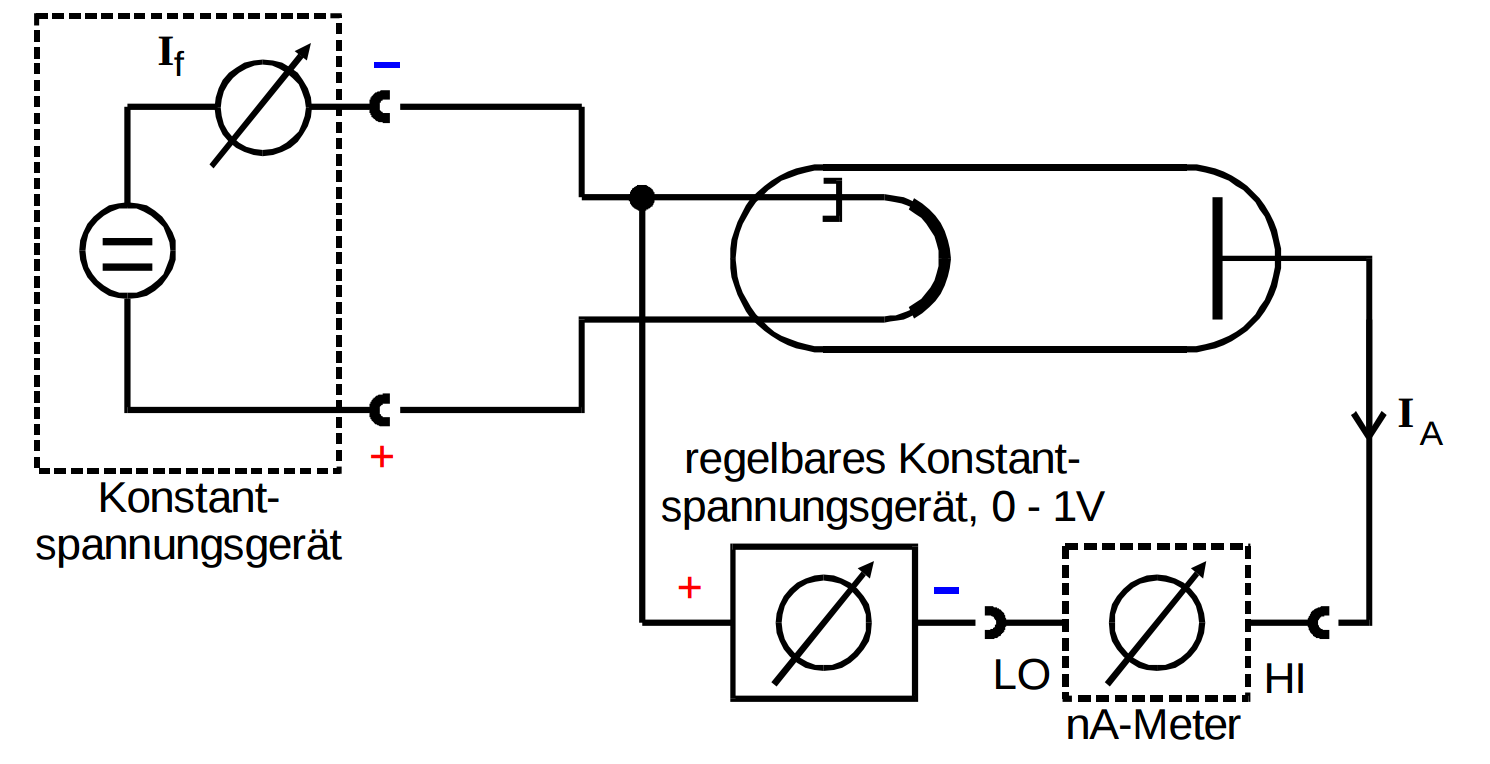
\includegraphics[width=0.9\textwidth]{V5042.png}
  \caption{Der Versuchsaufbau zur Aufnahme der Anlaufstromkurve. \cite{anleitung}}
  \label{fig:V5042}
\end{figure}
\noindent
Auch hier ist wieder ein Konstantspannungsgerät verbaut, welches für einen konstanten Heizstrom $I_f$ sorgt. Außerdem ist dieses erneut mit der Diode verbunden, welche allerdings nun mit einem Konstantspannunggerät verbunden ist, welches lediglich Spannungen zwischen \SI{0.1}{\volt} und \SI{0.96}{\volt} erzeugen kann. Außerdem ist die Diode mit einem Nanoampere-Meter verschaltet.
\subsection{Versuchsablauf}
\label{sec:ablauf}
Zuerst werden die Geräte, wie in Abbildung \ref{fig:V5041} dargestellt, verschaltet. Danach werden 5 mal 40 Werte für die Anodenspannung $U_A$ und für den Anodenstrom $I_A$ gemessen. $U_A$ befindet sich währendessen stets zwischen \SI{0}{\volt} und \SI{250}{\volt}. Die Heizspannung $U_f$ und der Heizstrom $I_f$ werden vor jedem Durchgang von 40 Messungen jeweils bestimmt und bleiben konstant. Danach werden 10 Werte für $I_A$ aufgenommen, um daraus unter anderem die Anlaufstromkurve zu bekommen. Dabei befindet sich $U_A$ währendessen stets zwischen \SI{0.1}{\volt} und \SI{0.96}{\volt}. Das Messgerät hat dabei einen Innenwiderstand von \SI{1}{\mega\ohm}.
\clearpage
\section{Auswertung}
\label{sec:auswertung}
Die in der Auswertung verwendeten Mittelwerte mehrfach gemessener Größen sind gemäß der
Gleichung
\begin{equation}
    \bar{x}=\frac{1}{n}\sum_{i=1}^n x_i
    \label{eq:mittelwert}
\end{equation}
bestimmt. Die Standardabweichung des Mittelwertes ergibt sich dabei zu
\begin{equation}
    \mathup{\Delta}\bar{x}=\sqrt{\frac{1}{n(n-1)}\sum_{i=1}^n\left(x_i-\bar{x}\right)^2}.
    \label{eq:standardabweichung}
\end{equation}
\subsection{Bestimmung von 5 Kennlinien}
Für die Bestimmung der 5 Kennlinien werden die in Tabelle \ref{tab:messwerte1}
stehenden Werte gemessen.
Diese werden dann in einem Graphen, welcher in Abbildung \ref{fig:plot1} zu
sehen ist, dargestellt. Der jeweils größte Wert wird dabei als
Sättigungsstrom $I_\mathup{S}$ angenommen.
\begin{figure}
  \centering
  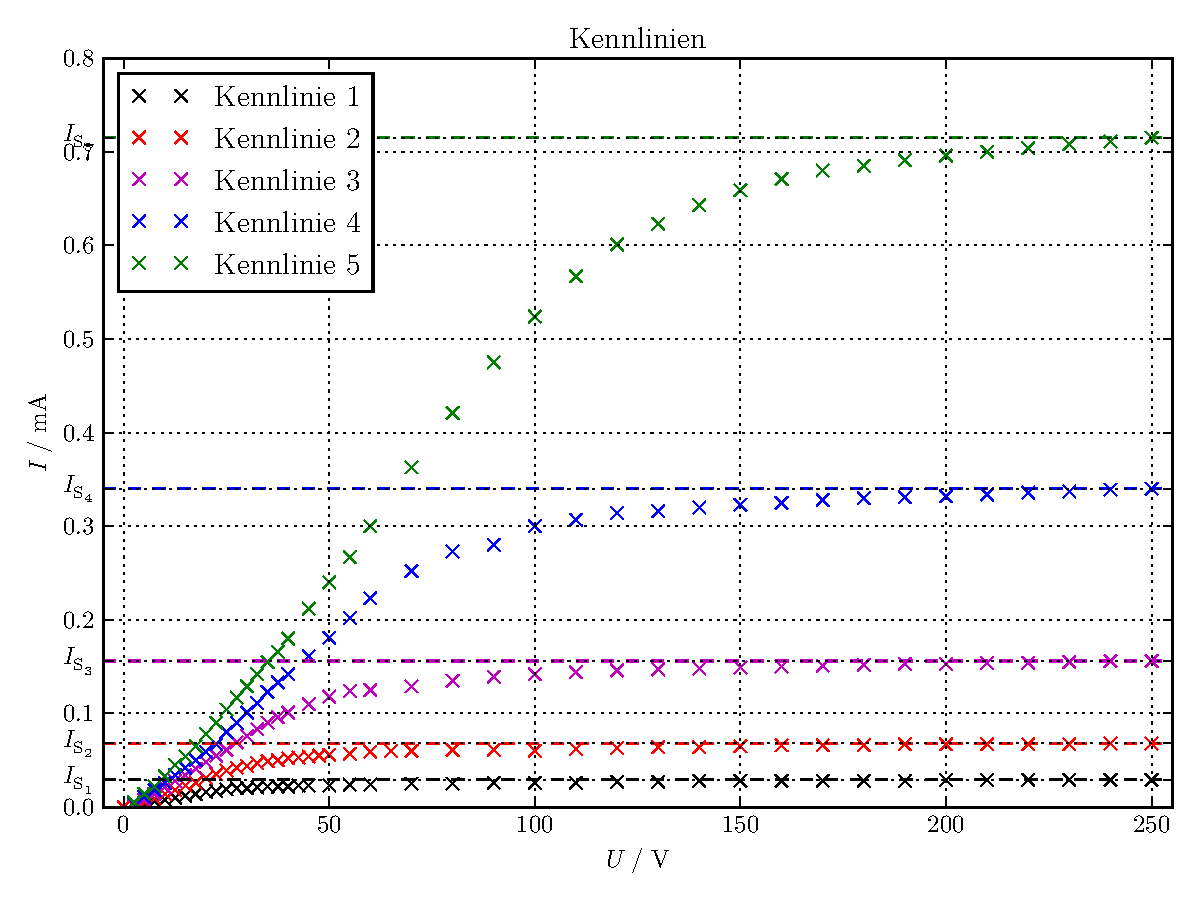
\includegraphics[width=\textwidth]{Plot.pdf}
  \caption{Gemessene Werte der Kennlinien.}
  \label{fig:plot1}
\end{figure}
\begin{table}
  \centering
  \sisetup{table-format=1.3}
  \begin{tabular}{S[table-format=3.1] S | S[table-format=3.1] S | S[table-format=3.1] S S S}
    \toprule
      \multicolumn{2}{c}{Kennlinie 1} & \multicolumn{2}{c}{Kennlinie 2} & \multicolumn{4}{c}{Kennlinien 3, 4 und 5} \\
      {$U_\mathup{A}$ in $\si{\volt}$} & {$I_\mathup{A}$ in $\si{\milli\ampere}$} & {$U_\mathup{A}$ in $\si{\volt}$} & {$I_\mathup{A}$ in $\si{\milli\ampere}$} & {$U_\mathup{A}$ in $\si{\volt}$} & {$I_\mathup{A}$ in $\si{\milli\ampere}$} & {$I_\mathup{A}$ in $\si{\milli\ampere}$} & {$I_\mathup{A}$ in $\si{\milli\ampere}$} \\
    \midrule
    0.0   & 0.000 &  0.0  & 0.000 &  0.0  & 0.000 & 0.000 & 0.000 \\
    2.5   & 0.001 &  2.5  & 0.001 &  2.5  & 0.003 & 0.004 & 0.005 \\
    5.0   & 0.003 &  5.0  & 0.005 &  5.0  & 0.008 & 0.011 & 0.014 \\
    7.5   & 0.006 &  7.5  & 0.009 &  7.5  & 0.014 & 0.018 & 0.022 \\
    10.0  & 0.008 & 10.0  & 0.014 & 10.0  & 0.021 & 0.026 & 0.033 \\
    12.5  & 0.010 & 12.5  & 0.018 & 12.5  & 0.028 & 0.034 & 0.045 \\
    15.0  & 0.012 & 15.0  & 0.023 & 15.0  & 0.034 & 0.042 & 0.054 \\
    17.5  & 0.014 & 17.5  & 0.026 & 17.5  & 0.041 & 0.050 & 0.065 \\
    20.0  & 0.016 & 20.0  & 0.031 & 20.0  & 0.048 & 0.059 & 0.078 \\
    22.5  & 0.017 & 22.5  & 0.035 & 22.5  & 0.055 & 0.067 & 0.090 \\
    25.0  & 0.019 & 25.0  & 0.039 & 25.0  & 0.061 & 0.080 & 0.104 \\
    27.5  & 0.020 & 27.5  & 0.042 & 27.5  & 0.069 & 0.090 & 0.117 \\
    30.0  & 0.020 & 30.0  & 0.044 & 30.0  & 0.076 & 0.101 & 0.129 \\
    32.5  & 0.021 & 32.5  & 0.047 & 32.5  & 0.083 & 0.111 & 0.142 \\
    35.0  & 0.022 & 35.0  & 0.049 & 35.0  & 0.090 & 0.123 & 0.155 \\
    37.5  & 0.022 & 37.5  & 0.050 & 37.5  & 0.096 & 0.133 & 0.166 \\
    40.0  & 0.022 & 40.0  & 0.052 & 40.0  & 0.101 & 0.142 & 0.180 \\
    42.5  & 0.023 & 42.5  & 0.053 & 45.0  & 0.110 & 0.161 & 0.212 \\
    45.0  & 0.023 & 45.0  & 0.054 & 50.0  & 0.118 & 0.181 & 0.240 \\
    50.0  & 0.023 & 47.5  & 0.055 & 55.0  & 0.124 & 0.202 & 0.267 \\
    55.0  & 0.024 & 50.0  & 0.056 & 60.0  & 0.125 & 0.223 & 0.300 \\
    60.0  & 0.024 & 55.0  & 0.057 & 70.0  & 0.129 & 0.252 & 0.363 \\
    70.0  & 0.025 & 60.0  & 0.059 & 80.0  & 0.135 & 0.273 & 0.421 \\
    80.0  & 0.025 & 65.0  & 0.060 & 90.0  & 0.139 & 0.280 & 0.475 \\
    90.0  & 0.026 & 70.0  & 0.060 & 100.0 & 0.142 & 0.300 & 0.524 \\
    100.0 & 0.026 & 80.0  & 0.061 & 110.0 & 0.144 & 0.307 & 0.567 \\
    110.0 & 0.026 & 90.0  & 0.061 & 120.0 & 0.146 & 0.314 & 0.601 \\
    120.0 & 0.027 & 100.0 & 0.060 & 130.0 & 0.147 & 0.316 & 0.623 \\
    130.0 & 0.027 & 110.0 & 0.062 & 140.0 & 0.148 & 0.320 & 0.643 \\
    140.0 & 0.028 & 120.0 & 0.063 & 150.0 & 0.149 & 0.323 & 0.659 \\
    150.0 & 0.028 & 130.0 & 0.064 & 160.0 & 0.150 & 0.325 & 0.671 \\
    160.0 & 0.028 & 140.0 & 0.064 & 170.0 & 0.151 & 0.328 & 0.680 \\
    170.0 & 0.028 & 150.0 & 0.065 & 180.0 & 0.152 & 0.330 & 0.685 \\
    180.0 & 0.028 & 160.0 & 0.066 & 190.0 & 0.153 & 0.331 & 0.691 \\
    190.0 & 0.028 & 170.0 & 0.066 & 200.0 & 0.153 & 0.332 & 0.696 \\
    200.0 & 0.029 & 180.0 & 0.066 & 210.0 & 0.154 & 0.334 & 0.700 \\
    210.0 & 0.029 & 190.0 & 0.067 & 220.0 & 0.154 & 0.336 & 0.704 \\
    220.0 & 0.029 & 200.0 & 0.067 & 230.0 & 0.155 & 0.337 & 0.708 \\
    230.0 & 0.029 & 210.0 & 0.067 & 240.0 & 0.156 & 0.339 & 0.711 \\
    240.0 & 0.029 & 220.0 & 0.067 & 250.0 & 0.156 & 0.340 & 0.715 \\
    250.0 & 0.029 & 230.0 & 0.067 &       &       &       &       \\
          &       & 240.0 & 0.068 &       &       &       &       \\
          &       & 250.0 & 0.068 &       &       &       &       \\
    \bottomrule
  \end{tabular}
  \caption{Gemessene Ströme und Spannungen.}
  \label{tab:messwerte1}
\end{table}
\clearpage
\noindent
Die Kennlinien wurden bei den in Tabelle \ref{tab:heiz} stehenden Heizspannungen
und Strömen gemessen.
\begin{table}
  \centering
  \caption{Gemessene Heizströme/Spannungen und Sättigungsströme.}
  \label{tab:heiz}
  \sisetup{table-format=1.2}
  \begin{tabular}{S S S[table-format=1.1] S[table-format=1.3]}
    \toprule
     & {$U_\mathup{f}$ in $\si{\volt}$} & {$I_\mathup{f}$ in $\si{\ampere}$} & {$I_\mathup{S}$ in $\si{\milli\ampere}$} \\
    \midrule
    \text{Kennlinie 1} & 3.25 & 1.8 & 0.029 \\
    \text{Kennlinie 2} & 3.5  & 1.9 & 0.068 \\
    \text{Kennlinie 3} & 4.0  & 2.0 & 0.156 \\
    \text{Kennlinie 4} & 4.25 & 2.1 & 0.340 \\
    \text{Kennlinie 5} & 4.5  & 2.2 & 0.715 \\
    \bottomrule
  \end{tabular}
\end{table}
\subsection{Betrachtung der Strom-Spannungs-Beziehung nach dem Langmuir-Schottkyschen Gesetz}
Für diese Betrachtung werden die gemessenen Werte der fünften Kennlinie verwendet.
Diese werden doppelt-logarithmisch aufgetragen und anschließend mit der Funktion
curve-fit von Python eine Anpassung an eine lineare Funktion
\begin{equation}
  f(x) = m \cdot x + b
  \label{eqn:linear}
\end{equation}
durchgeführt. Hierzu werden nur die ersten 23 Werte verwendet, da bei den darauf
folgenden Werten das Langmuir-Schottkysche Gesetz nicht mehr gültig ist.
Dabei ergeben sich die folgenden Parameter:
\begin{align*}
  m &= \SI{1.254(9)}{} \\
  b &= \SI{-6.33(3)}{}
\end{align*}
Die Steigung $m$ der Geraden steht für den Exponenten der Spannung in Formel \eqref{eqn:raumladung}.
In Abbildung \ref{fig:plot2} ist der entsprechende Graph zu sehen.
\begin{figure}[H]
  \centering
  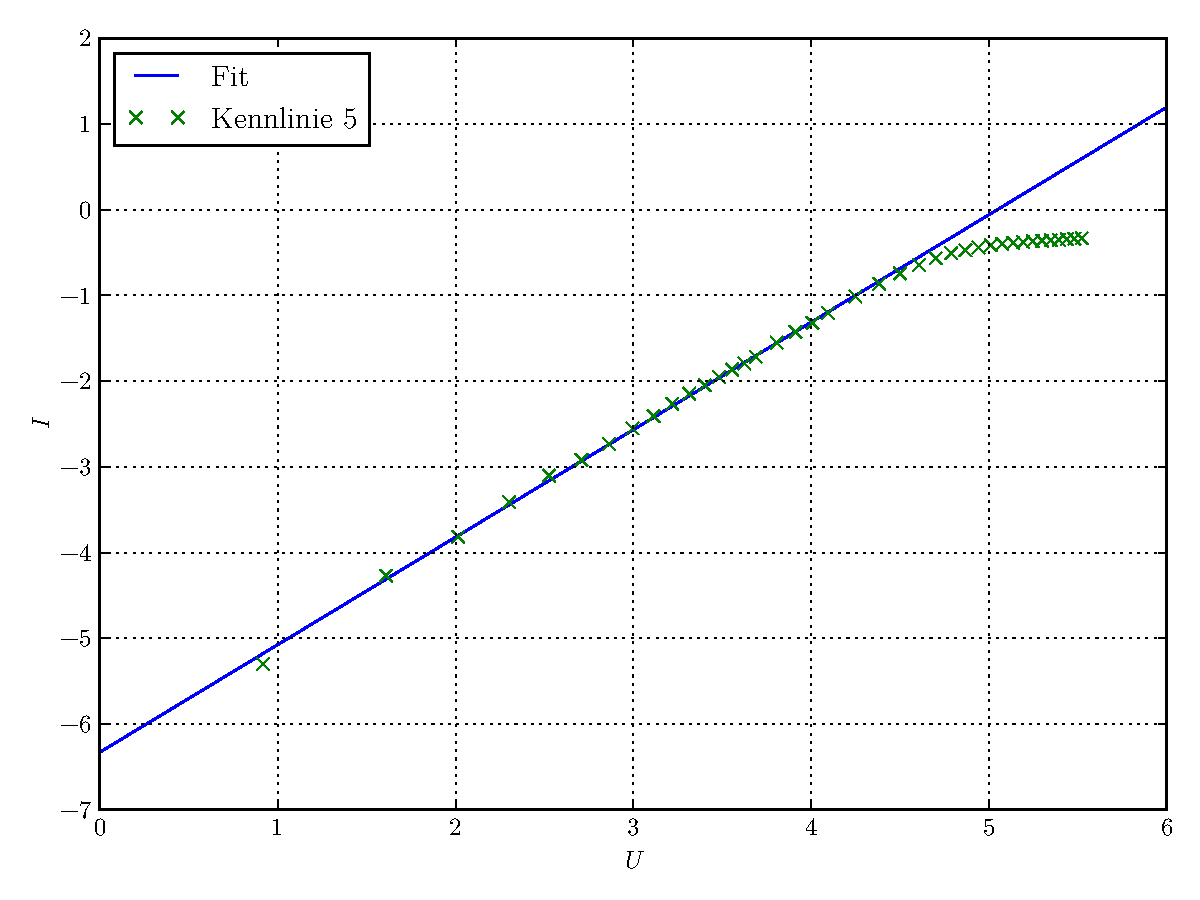
\includegraphics[width=0.9\textwidth]{Plot2.pdf}
  \caption{Logarithmierte Werte der fünften Kennlinie und Fit.}
  \label{fig:plot2}
\end{figure}
\subsection{Bestimmung der Kathodentemperatur mittels Messung des Anlaufstromgebiets}
Bei der Messung des Anlaufstromgebiets werden die in Tabelle \ref{tab:messwerte2}
stehenden Werte gemessen. Dabei wird eine Heizspannung von $\SI{4.5}{\volt}$
verwendet. Da das Messgerät für den Strom einen Innenwiderstand von $\SI{1}{\mega\ohm}$
besitzt muss die Spannung zunächst noch korrigiert werden. Hierzu wird der Strom
nach dem Ohmschen Gesetz mit dem Widerstand multipliziert und anschließend
dieser Wert von der gemessenen Spannung abgezogen.
\begin{table}
  \centering
  \caption{Gemessene Spannungen und Ströme.}
  \label{tab:messwerte2}
  \sisetup{table-format=1.2}
  \begin{tabular}{S S[table-format=1.3]}
    \toprule
    {$U_\mathup{A}$ in $\si{\volt}$} & {$I_\mathup{A}$ in $\si{\nano\ampere}$} \\
    \midrule
    0.0  & 8.4   \\
    0.1  & 4.6   \\
    0.2  & 2.5   \\
    0.3  & 1.45  \\
    0.4  & 0.85  \\
    0.5  & 0.5   \\
    0.6  & 0.3   \\
    0.7  & 0.22  \\
    0.8  & 0.165 \\
    0.9  & 0.13  \\
    0.96 & 0.115 \\
    \bottomrule
  \end{tabular}
\end{table}
\noindent
Diese Werte werden nun logarithmisch aufgetragen und erneut eine Anpassung an
eine lineare Funktion \eqref{eqn:linear} durchgeführt. Der entsprechende Graph
ist in Abbildung \ref{fig:plot3} dargestellt.
\begin{figure}[H]
  \centering
  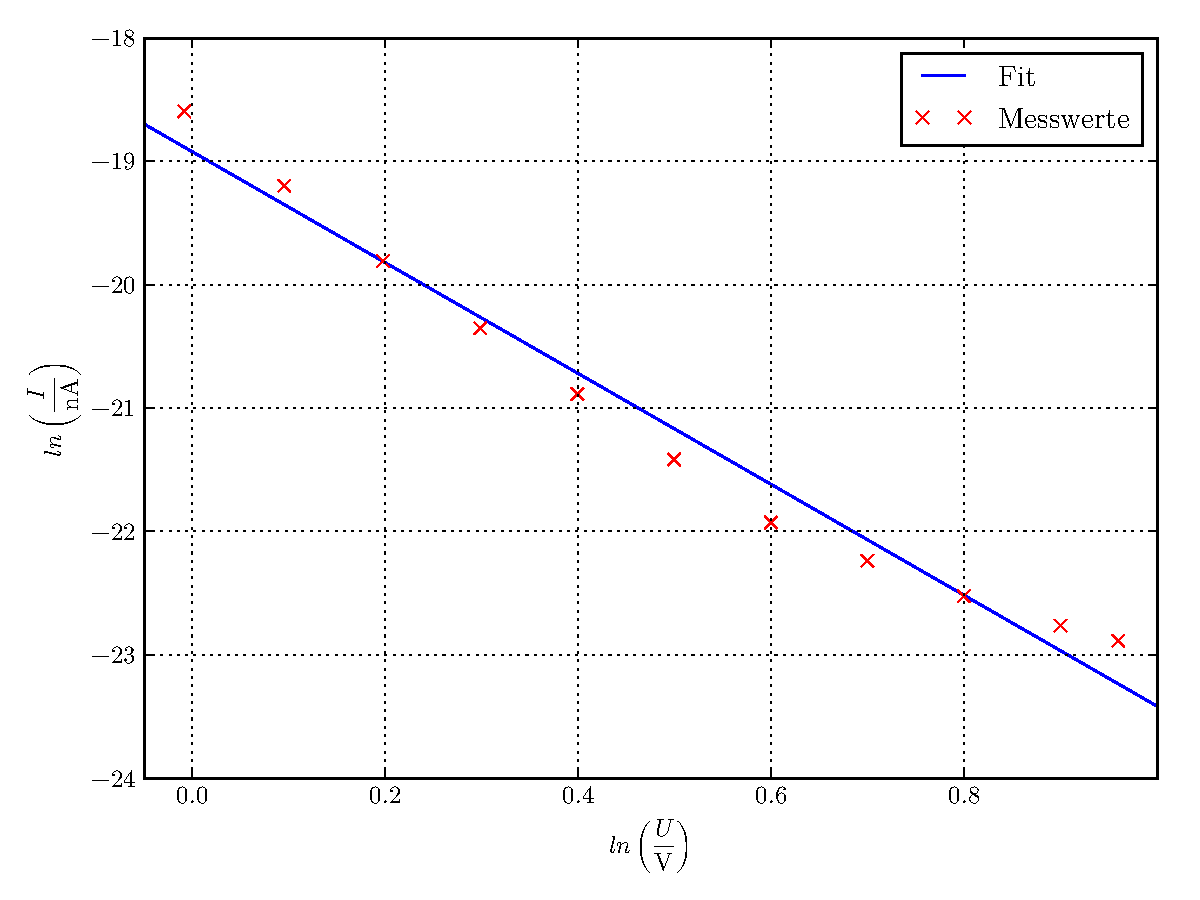
\includegraphics[width=\textwidth]{Plot3.pdf}
  \caption{Logarithmierte Werte des Anlaufstromgebiets und Fit.}
  \label{fig:plot3}
\end{figure}
\noindent
Als Parameter ergeben sich:
\begin{align*}
  m &= \SI{-4.5(2)}{} \\
  b &= \SI{-18.9(1)}{}
\end{align*}
Über die Steigung und den Exponenten von Formel \eqref{eqn:stromdichte} lässt
sich dann die Kathodentemperatur bestimmen:
\begin{equation}
  T = -\frac{e_0}{k \cdot m} = \SI{2582(130)}{\kelvin}
\end{equation}
Dabei werden für $e_0$ und $k$ die bei Scipy \cite{scipy} enthaltenen Werte der Elementarladung
und der Boltzmann-Konstante verwendet. ($e_0 \approx \SI{1.602e-19}{\coulomb}$, $k \approx \SI{1.381e-23}{\joule\per\kelvin}$)
\subsection{Bestimmung der Kathodentemperatur über die Leistungsbilanz}
Für die Abschätzung der Kathodentemperatur werden die fünf Heizspannungen und
Ströme aus der ersten Messung verwendet. Diese stehen mit den sich daraus nach
\begin{equation}
  N = U \cdot I
\end{equation}
ergebenden zugeführten Leistungen in Tabelle \ref{tab:leist}.
\begin{table}
  \centering
  \caption{Gemessene Heizströme/Spannungen und Leistungen.}
  \label{tab:leist}
  \sisetup{table-format=1.2}
  \begin{tabular}{S S S[table-format=1.1] S[table-format=1.3]}
    \toprule
     & {$U_\mathup{f}$ in $\si{\volt}$} & {$I_\mathup{f}$ in $\si{\ampere}$} & {$N_\mathup{zu}$ in $\si{\watt}$} \\
    \midrule
    \text{Kennlinie 1} & 3.25 & 1.8 & 5.850 \\
    \text{Kennlinie 2} & 3.5  & 1.9 & 6.650 \\
    \text{Kennlinie 3} & 4.0  & 2.0 & 8.000 \\
    \text{Kennlinie 4} & 4.25 & 2.1 & 8.925 \\
    \text{Kennlinie 5} & 4.5  & 2.2 & 9.900 \\
    \bottomrule
  \end{tabular}
\end{table}
Die Formel für die Leistungsbilanz lautet:
\begin{equation}
  N_\mathup{zu} = N_\mathup{Str} + N_\mathup{WL}.
  \label{eqn:leistungsbil}
\end{equation}
$N_\mathup{Str}$ ist mit
\begin{equation}
  N_\mathup{Str} = f \eta \sigma T^4
  \label{eqn:strahlungsleistung}
\end{equation}
gegeben. Damit lässt sich die Leistungsbilanz auch als
\begin{equation}
  N_\mathup{zu} = f \eta \sigma T^4 + N_\mathup{WL}
  \label{eqn:leistungsbil2}
\end{equation}
schreiben. $N_\mathup{WL}$ muss abgeschätzt werden.
In disem Fall wird dafür ein Wert von $\SI{0.95}{\watt}$ verwendet.
Die Fläche $f$ der Diode beträgt $\SI{0.32}{\square\centi\meter}$.
$\eta$ ist mit 0.28 und $\sigma$ mit $\SI{5.7e-12}{\watt\per\square\centi\meter\per\kelvin\tothe4}$
gegeben. Schließlich wird die Gleichung nach T umgeformt um die Temperatur zu
erhalten.
\begin{equation}
  T = \left(\frac{N_\mathup{zu} - N_\mathup{WL}}{f \eta \sigma}\right)^\frac{1}{4}
  \label{eqn:tempkath}
\end{equation}
Die Ergebnisse der Rechnung für die fünf Heizspannungen stehen in Tabelle \ref{tab:ergebn}
\begin{table}[H]
  \centering
  \caption{Gemessene Heizspannungen, Sättigungsströme und Temperaturen.}
  \label{tab:ergebn}
  \sisetup{table-format=1.2}
  \begin{tabular}{S S S[table-format=1.3] S[table-format=4.0]}
    \toprule
     & {$U_\mathup{f}$ in $\si{\volt}$} & {$I_\mathup{S}$ in $\si{\milli\ampere}$} & {$T$ in $\si{\kelvin}$} \\
    \midrule
    \text{Kennlinie 1} & 3.25 & 0.029 & 1760 \\
    \text{Kennlinie 2} & 3.5  & 0.068 & 1828 \\
    \text{Kennlinie 3} & 4.0  & 0.156 & 1928 \\
    \text{Kennlinie 4} & 4.25 & 0.340 & 1988 \\
    \text{Kennlinie 5} & 4.5  & 0.715 & 2046 \\
    \bottomrule
  \end{tabular}
\end{table}
\subsection{Bestimmung der Austrittsarbeit}
Zur Bestimmung der Austrittsarbeit wir Formel \eqref{eqn:richardson}
nach $e_0 \phi$ aufgelöst.
Sie lautet dann:
\begin{equation}
  e_0 \phi = \ln \left( \frac{j_\mathup{S} \cdot h^3}{4 \pi \cdot e_0 m_0 k^2 T^2} \right) \cdot k T
  \label{eqn:austritt}
\end{equation}
Da in der Formel von der Sättigungsstromdichte $j_\mathup{S}$ die Rede ist
muss der von uns gemessene Sättigungsstrom $I_\mathup{S}$ noch durch die Fläche
geteilt werden. Dabei ist auf die Einheiten zu achten. Für die Elementarladung
$e_0$, die Elektronenmasse $m_0$ ($\approx \SI{9.109e-31}{\kilo\gram}$), die Boltzmann-Konstante $k$ und die Planksche
Konstante $h$ ($\approx \SI{6.626e-34}{\joule\second}$) werden die Werte von Scipy \cite{scipy} verwendet.
Damit ergeben sich die in Tabelle \ref{tab:ergebnissephi} stehenden
Austrittsarbeiten.
\begin{table}[H]
  \centering
  \caption{Gemessene Heizspannungen, Sättigungsströme und Austrittsarbeiten.}
  \label{tab:ergebnissephi}
  \sisetup{table-format=1.2}
  \begin{tabular}{S S S[table-format=2.3] S S}
    \toprule
     & {$U_\mathup{f}$ in $\si{\volt}$} & {$j_\mathup{S}$ in $\si{\milli\ampere}$} & {$e_0 \phi$ in $\SI{e-19}{\joule}$} & {$e_0 \phi$ in $\si{\electronvolt}$} \\
    \midrule
    \text{Kennlinie 1} & 3.25 & 0.906 & 7.06 & 4.41 \\
    \text{Kennlinie 2} & 3.5  & 2.125 & 7.13 & 4.45 \\
    \text{Kennlinie 3} & 4.0  & 4.875 & 7.33 & 4.58 \\
    \text{Kennlinie 4} & 4.25 & 10.625 & 7.36 & 4.60 \\
    \text{Kennlinie 5} & 4.5  & 22.344 & 7.38 & 4.61 \\
    \bottomrule
  \end{tabular}
\end{table}
Die Austrittsarbeit wird anschließend zu
\begin{equation}
  e_0 \phi = \SI{4.53(4)}{\electronvolt}
\end{equation}
gemittelt.
\clearpage
\section{Diskussion}
\label{sec:diskussion}
In Tabelle \ref{tab:ergebnissevers} stehen die Ergebnisse des Versuchs.
\begin{table}[H]
  \centering
  \caption{Ergebnisse.}
  \label{tab:ergebnissevers}
  \sisetup{table-format=1.1}
  \begin{tabular}{S S S}
    \toprule
    {Größe} & {Ergebniss} & {Theoriewert} \\
    \midrule
    $I_\mathup{S_1}$ & $\SI{0.029}{\milli\ampere}$ & / \\
    $I_\mathup{S_2}$ & $\SI{0.068}{\milli\ampere}$ & / \\
    $I_\mathup{S_3}$ & $\SI{0.156}{\milli\ampere}$ & / \\
    $I_\mathup{S_4}$ & $\SI{0.340}{\milli\ampere}$ & / \\
    $I_\mathup{S_5}$ & $\SI{0.715}{\milli\ampere}$ & / \\
    $V^x$ & $\SI{1.254(9)}{}$ & 1.5 \\
    $T_{\SI{4.5}{\volt}} \text{(Methode 1)}$ & $\SI{2582(130)}{\kelvin}$ & / \\
    $T_{\SI{3.25}{\volt}} \text{(Methode 2)}$ & $\SI{1760}{\kelvin}$ & / \\
    $T_{\SI{3.5}{\volt}} \text{(Methode 2)}$ & $\SI{1828}{\kelvin}$ & / \\
    $T_{\SI{4.0}{\volt}} \text{(Methode 2)}$ & $\SI{1928}{\kelvin}$ & / \\
    $T_{\SI{4.25}{\volt}} \text{(Methode 2)}$ & $\SI{1988}{\kelvin}$ & / \\
    $T_{\SI{4.5}{\volt}} \text{(Methode 2)}$ & $\SI{2046}{\kelvin}$ & / \\
    $\phi$ & $\SI{4.53(4)}{\electronvolt}$ & $\SI{4.54}{\electronvolt}$ \cite{austritt} \\
    \bottomrule
  \end{tabular}
\end{table}
\noindent
Die erhaltenen Kurven der Kennlinien passen gut zu dem Schema aus Abbildung \ref{fig:V5044}.
Der bestimmte Exponent der Spannungsabhängigkeit von Formel \eqref{eqn:raumladung}
liegt etwas unterhalb von dem Theoriewert, was an einem systematischen Fehler liegen
dürfte, da der statistische Fehler der Steigung kleiner ist als die Abweichung.
Ein derartiger Fehler wäre z.B. ein ungenaues Ablesen der Werte. Außerdem ist
während dem Versuch aufgefallen, dass teilweise bei einem bestimmten Wert auf
der Skala der Spannung ein keliner Sprung stattfand, nachdem sich für davor
gemessene Werte bei erneutem Messen ein etwas höherer Wert ergab. Somit könnte
auch durch die Messgeräte ein Fehler zustande kommen.

\noindent
Beim Vergleich der bestimmten Temperaturen fällt eine größere Differenz zwischen
den beiden Werten für $\SI{4.5}{\volt}$ auf. Da das Ergebnis der Austrittsarbeit
sehr gut ist und den Theoriewert einschließt sollten die dazu verwendeten
Ergebnisse für die Sättigungsströme sowie die mit Methode 2 bestimmten
Temperaturen ebenfalls sehr gut passen. Daraus lässt sich schließen, dass die
Bestimmung der Temperatur nach der ersten Methode weniger genau ist. Der
statistische Fehler ist mit $\SI{130}{\kelvin}$ schon groß.

\noindent
Wie bereits erwähnt liegt der bestimmte Wert der Austrittsarbeit $e_0 \phi$
sehr dicht an dem Theoriewert.
Insgesamt ist der Versuch einfach durchzuführen und liefert gute Ergebnisse.
\clearpage
\nocite{*}
\printbibliography
\end{document}
